\chapter{MODELAGEM DO ESCOAMENTO SANGUÍNEO}\label{sec:modelagem_escoamento}

%\textcolor{red}{IGOR: está errada a citação do trabalho do método de Duan e Zamir (1995), não é a citação que colocou \cite{Duan}.} \textcolor{green}{OK}

Neste capítulo, apresenta-se o modelo matemático de Duan e Zamir \cite{Duan1992}, para o escoamento sanguíneo pulsátil em árvores arteriais \igunew{que será utilizado para desenvolver a ferramenta computacional}. Por fim, apresenta um algoritmo que \igunew{resume} passos dos cálculos realizados para obtenção da pressão e fluxo ao longo da árvore arterial.

%--------------------------------------------------------------------------------%
\section{MODELO MATEMÁTICO}\label{sec:modelo_matematico}

A propagação de ondas em um tubo é governada pela equações da onda para a pressão $p(x,t)$ e fluxo $q(x,t)$ como seguem:
\begin{eqnarray}
	\frac{\partial q}{\partial t} &=& -cY \frac{\partial p}{\partial x},
	\label{01_p}\\
	\frac{\partial p}{\partial t} &=& -\frac{c}{Y} \frac{\partial q}{\partial x}, 
	\label{02_q}
\end{eqnarray}
nos quais $t$ é o tempo, $x$ é a coordenada axial ao longo do tubo, $c$ é a velocidade de onda, $Y = \frac{A}{\rho c}$ é a admitância e $A$ é a área da seção transversal do tubo, e $\rho$ é a densidade do fluido. Estas equações são baseadas na linearização das equações de movimento do fluido \cite{Fung,Lighthill}. 

Para uma onda harmônica simples, as Equações (\ref{01_p}) e (\ref{02_q}) resultam em:
\begin{eqnarray}
	p &=& \bar{p}_0 \exp\left[i\omega\left(t - \frac{x}{c}\right)\right] + R  \bar{p}_0 \exp\left[i\omega\left(t - \frac{2L}{c} + \frac{x}{c}\right)\right],
	\label{03_p}\\
	q &=& Y\left\{\bar{p}_0 \exp\left[i\omega\left(t - \frac{x}{c}\right)\right] -  R  \bar{p}_0 \exp\left[i\omega\left(t - \frac{2L}{c} + \frac{x}{c}\right)\right]\right\},
	\label{04_1}
\end{eqnarray}
onde $\omega = 2 \pi f$ é a frequência angular, $f$ é frequência em Hertz, $L$ é o comprimento do tubo, $\bar{p}_0$ é a amplitude da onda incidente, $R$ é o coeficiente de reflexão definido pela razão entre as ondas refletidas pelas ondas que chegam no local de reflexão \cite{Fung,Karreman} e $i$ é a unidade imaginária ($i^2 = -1$).

\igunew{O modelo matemático considera que o segmento é composto pelo nó proximal $A$ e pelo nó distal $B$, considerando o nó proximal o ponto mais próximo da origem do fluxo e o nó distal o ponto mais distante, como apresentado na Figura~\ref{fig:proximaldistal}.}

\begin{figure}[!htbp]
	\centering
	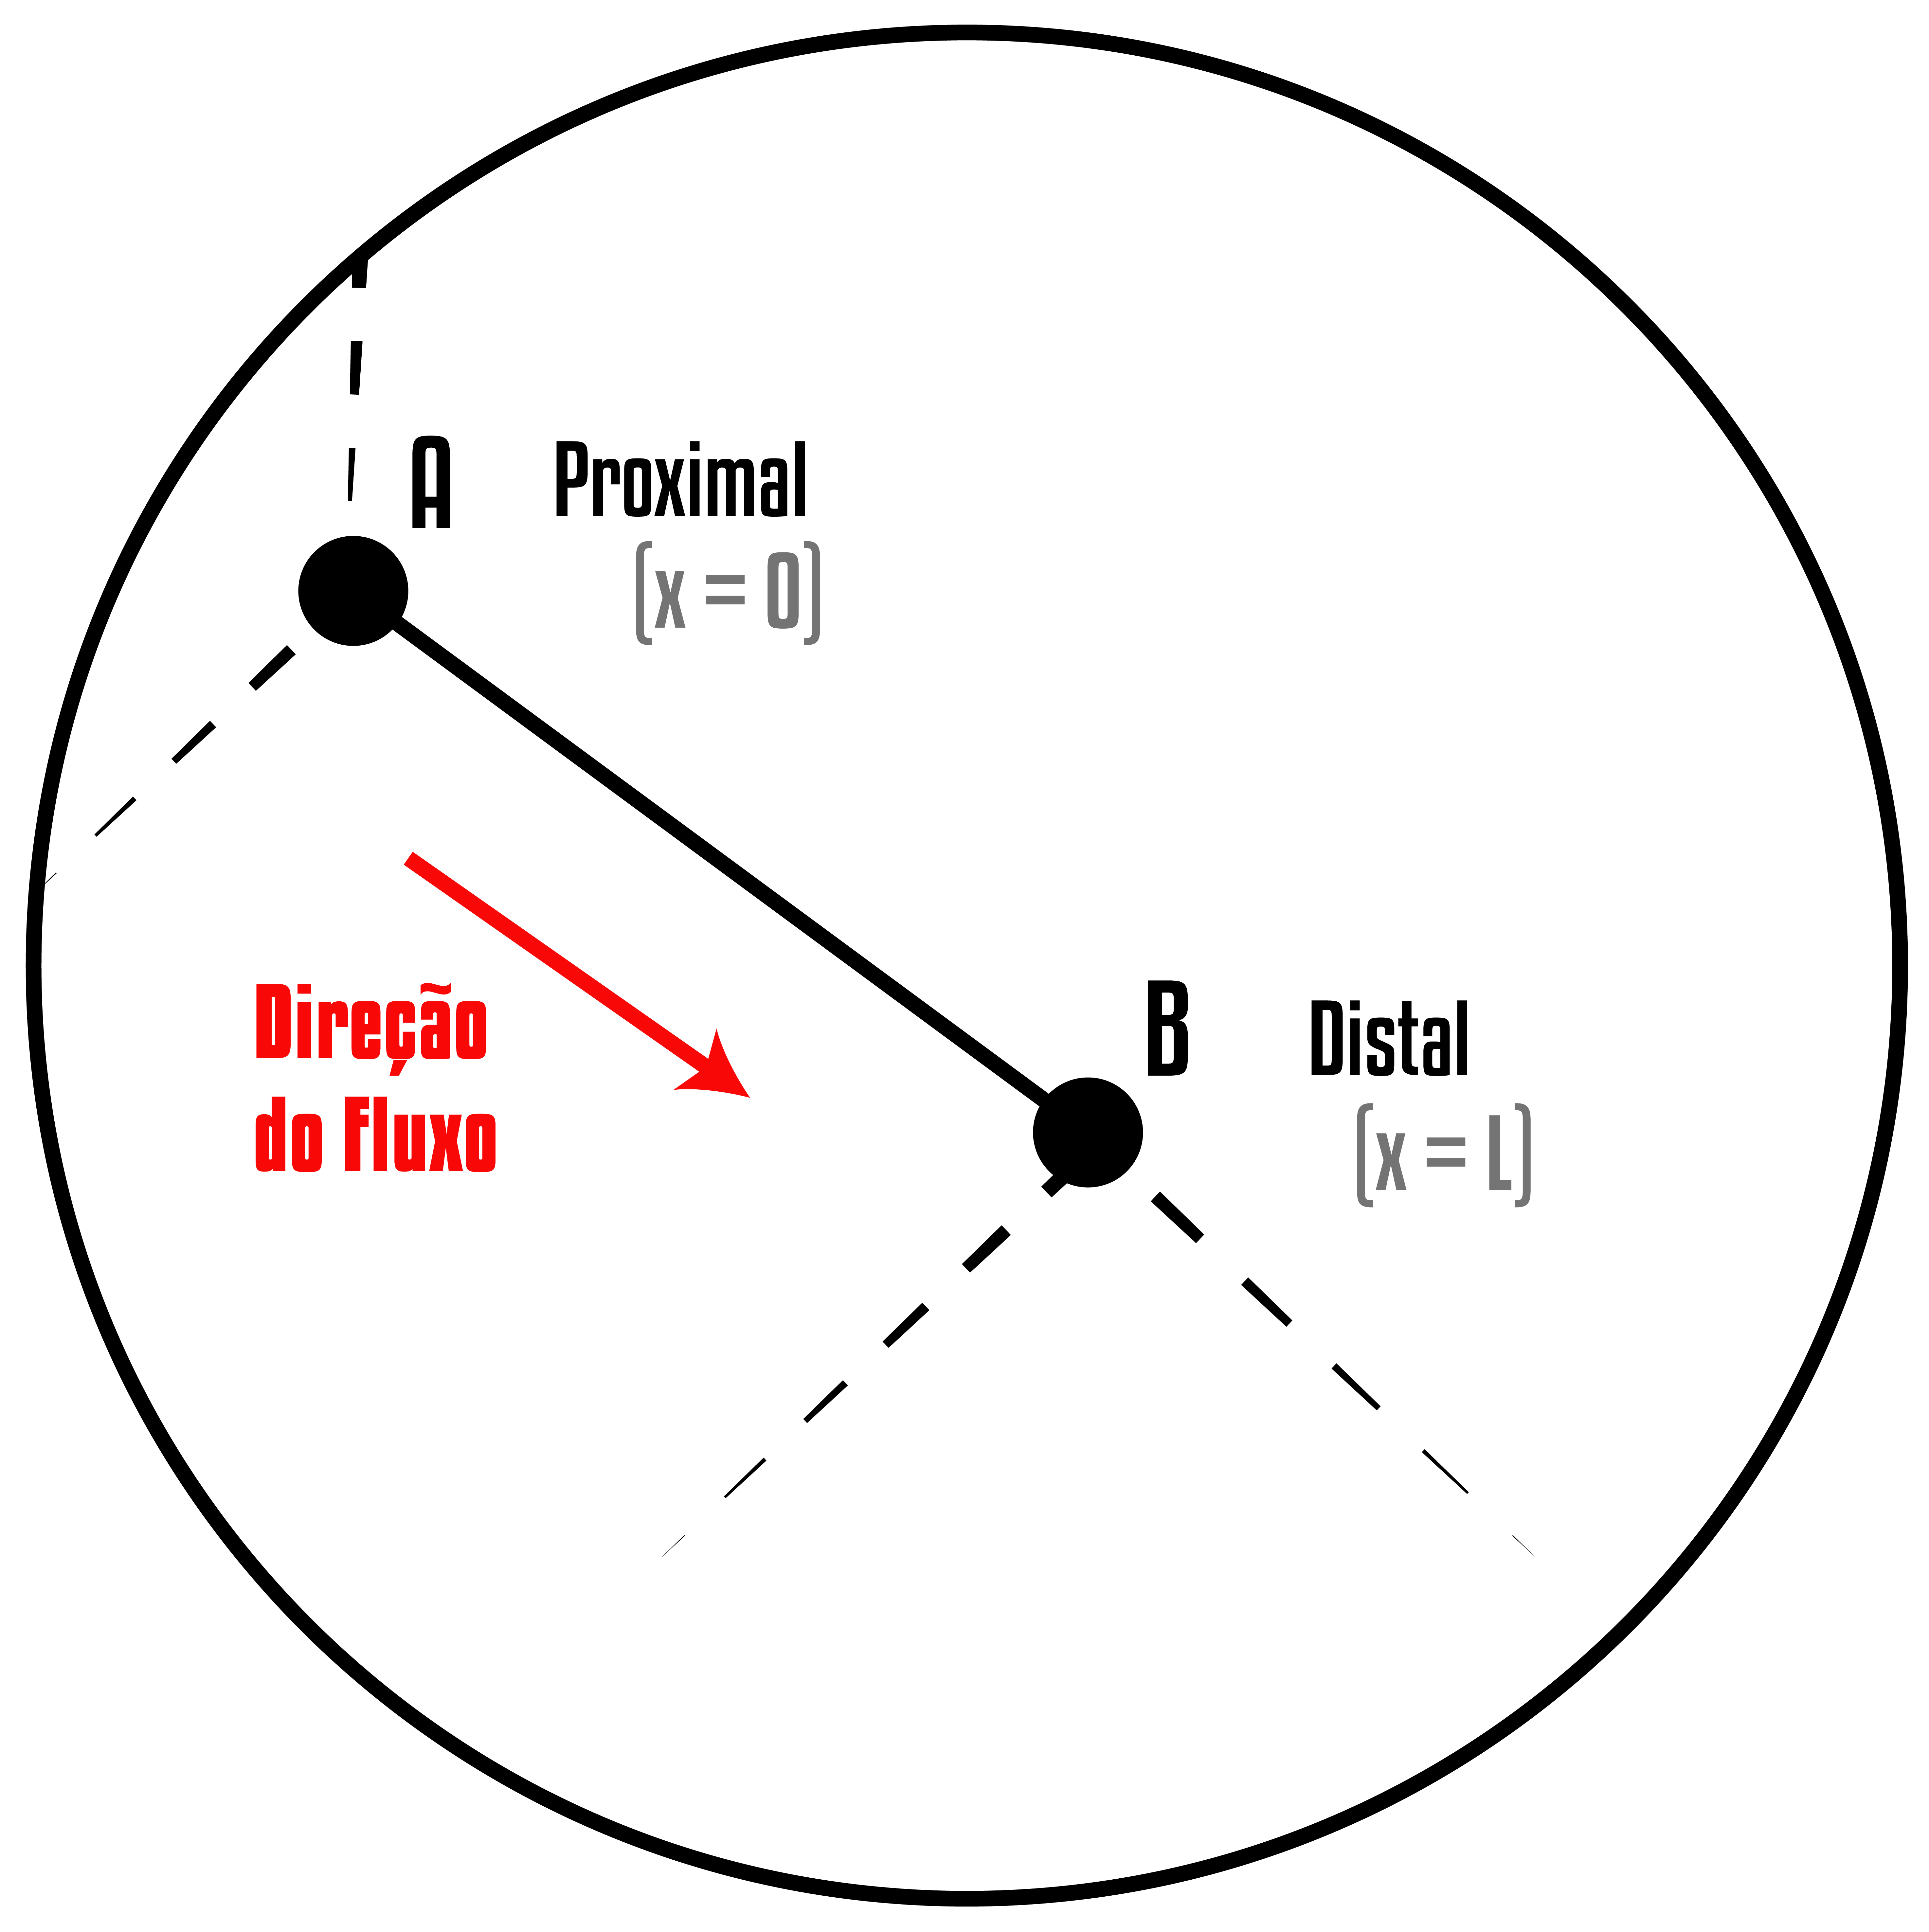
\includegraphics[scale=1]{Figures/ProximalDistal@16x.png}
	\caption{Segmento do modelo geométrico de uma árvore arterial, composto pelo nó proximal $A$ e pelo nó distal $B$.}
	\label{fig:proximaldistal}
\end{figure}

As Equações \eqref{03_p} e \eqref{04_1} para pressão e fluxo são aplicadas em cada segmento de vaso do modelo de árvore arterial, tomando $x = 0$ para o nó proximal e $x = L$ para o nó distal do segmento. Um segmento de vaso é definido pelo intervalo vascular entre dois locais de ramificação \cite{Zamir3}. No sistema arterial, as bifurcações são os locais de ramificação mais comuns~\cite{Zamir1}.

De~\citeyear{Duan}~\citeauthoronline{Duan}, um segmento de vaso é identificado por $(k,j)$, onde o $k$ representa o nível da geração e $j$ representa a ordem do segmento naquela geração, como na Figura~\ref{fig1:arterial-tree}. Desta forma, a pressão e o fluxo ao longo de um segmento  $(k,j)$ do modelo de árvore arterial são dados por:
\begin{eqnarray}
	p(k,j) &=& \bar{p}(k,j) \exp\left[i\omega\left(t - \frac{x(k,j)}{c(k,j)}\right)\right] \nonumber \\
	&+& R(k,j)  \bar{p}(k,j) \exp\left[i\omega\left(t - \frac{2L(k,j)}{c(k,j)} + \frac{x(k,j)}{c(k,j)}\right)\right],
	\label{05_p}\\
	q (k,j) &=& Y(k,j)\left\{\bar{p}(k,j) \exp\left[i\omega\left(t - \frac{x(k,j)}{c(k,j)}\right)\right]\right. \nonumber \\
	&-& \left. R(k,j)  \bar{p}(k,j) \exp\left[i\omega\left(t - \frac{2L(k,j)}{c(k,j)} + \frac{x(k,j)}{c(k,j)}\right)\right]\right\},
	\label{06_q}
\end{eqnarray}
nos quais $\bar{p}(k,j)$ é a amplitude combinada do grupo de ondas progressivas no segmento $(k,j)$ e $R(k,j)$ é o coeficiente de reflexão no final daquele segmento. \igunew{O coeficiente de reflexão $R$ é a razão das ondas progressivas pelas ondas atrasadas avaliadas no nó distal $x(k,j) = L(k,j)$. }

O grupo de ondas progressivas viaja no sentido positivo de $x(k,j)$, estas são compostas de ondas progressivas vindo de vasos acima deste, bem como, ondas refletidas na junção à montante $x(k,j) = 0$. O grupo de ondas atrasadas viaja no sentido oposto e é composto por ondas vindas de vasos conectados ao nó distal, estas ondas são refletidas na junção à jusante $x(k,j) = L(k,j)$\igunew{, estas ondas viajam na direção oposta ao fluxo sanguíneo e são consideradas a reflexão  das ondas progressivas nos segmentos adjacentes ao nó distal $B$}. 

As Equações \eqref{05_p} e \eqref{06_q} descrevem, respectivamente, as ondas de pressão e de fluxo localmente em um segmento $(k,j)$ do modelo de árvore, e localmente na posição $x(k,j)$ dentro deste segmento de vaso. \igunew{O principal objetivo deste modelo matemático é determinar as duas variáveis desconhecidas: a amplitude da pressão  $\bar{p} (k,j)$} e o coeficiente de reflexão $R (k,j)$, que são detalhados na Seção~\ref{sec:pressao-fluxo}. 

A Figura~\ref{fig1:arterial-tree} mostra a notação usada para identificar cada segmento de vaso $(k,j)$, onde $k$ é a geração/nível do vaso e $j$ é um número sequencial dentro daquela geração. Os nós proximal e distal do segmento $(k,j)$~\ref{fig:proximaldistal} são denotados por $A$ e $B$, respectivamente. O coeficiente de reflexão $R(k,j)$ do segmento $(k,j)$ está associado ao nó distal $B$.

Na Equação~\eqref{06_q}, tem-se a admitância característica para cada segmento dada por:
\begin{equation}
	Y(k,j) = \frac{A(k,j)}{\rho(k,j)c(k,j)},
	\label{eq:admitancia}
\end{equation}
nos quais $A(k,j)$ é a área da seção transversal do segmento $(k,j)$, $\rho(k,j)$ é a densidade do fluido dentro do vaso e $c(k,j)$ é a velocidade da onda correspondente. A admitância de um segmento é uma medida do quanto o segmento permite o fluxo.

Assumindo um segmento elástico de parede fina, a velocidade da onda $c(k,j)$ é calculada
por~\cite{Fung}:
\begin{equation}
	c(k,j) = \sqrt{\frac{E(k,j) h(k,j)}{\rho(k,j) d(k,j)}},\label{eq:velocidade}
\end{equation}
onde $E(k,j)$ é o módulo de Young, $d(k,j)$ é o diâmetro do segmento $(k,j)$ e $h(k,j)$ é a espessura da parede do segmento, a qual neste estudo é dada por~\cite{Duan}: 
\begin{equation}
	h(k,j) = 0,05 d(k,j).
\end{equation}

\begin{figure}[h] 
	\begin{center}
		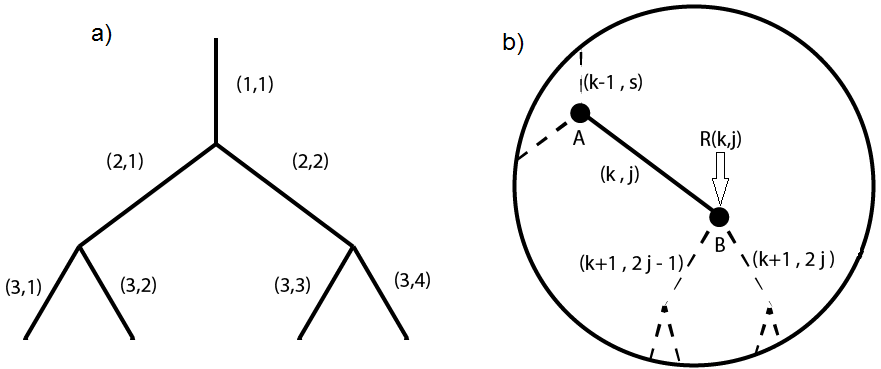
\includegraphics[scale = 0.5]{Figures/ArterialTree_Zamir.png}%
		\caption{Notação usada para identificar cada segmento de vaso $(k,j)$ (figura adaptada de~\citeyear{Duan}~\citeauthoronline{Duan}). }
		\label{fig1:arterial-tree}%
	\end{center}
\end{figure}

%--------------------------------------------------------------------------------%
\subsection{CÁLCULO DA PRESSÃO E DO FLUXO SANGUÍNEO}\label{sec:pressao-fluxo}

Para determinar a pressão $\bar{p} (k,j)$ em um certo segmento $(k,j)$, aplica-se a condição de continuidade de pressão no nó proximal $A$ (ver Figura \ref{fig1:arterial-tree}). Escrevendo as componentes progressiva e atrasada da onda como $p_f (k,j)$ e $p_b (k,j)$ respectivamente, a pressão na posição proximal do segmento  $x(k,j) = 0$ é dada por:
\begin{equation}
	\left[ p (k,j) \right]_A = \left[ p_f (k,j) \right]_A + \left[ p_b (k,j)\right]_A,
	\label{09_p}
\end{equation}
nos quais as pressões $\left[ p_f(k,j) \right]_A$ e $\left[ p_b(k,j) \right]_A$ são expressas por:
\begin{eqnarray}
	\left[ p_f(k,j) \right]_A &=& \bar{p}(k,j)\exp\left[ i\omega t\right],
	\label{10_p_f}\\
	\left[ p_b (k,j) \right]_A &=& R(k,j)\bar{p}(k,j)\exp\left[i\omega \left(t - \frac{2L(k,j)}{c(k,j)}\right) \right].
	\label{11_p_b}
\end{eqnarray}
Similarmente, a pressão no segmento pai $(k-1,s)$ pode ser escrita como:
\begin{equation}
	p(k-1,s) =  p_f(k-1,s) + p_b (k-1,s),
	\label{12_p|_f}
\end{equation}
nos quais $s$ é um número sequencial do segmento pai e as pressões $ p_f (k-1,s)$ e $p_b (k-1,s)$ são dadas por:
\begin{eqnarray}
	p_f (k-1,s) &=& \bar{p}(k-1,s)\exp\left[i\omega \left(t - \frac{x(k-1,s)}{c (k-1,s)}\right) \right],\\
	\label{13_p_f}
	p_b (k-1,s) &=& R (k-1,s)\bar{p}(k-1,s)\exp\left[ i\omega \left( t - \frac{2L(k-1,s)}{c(k-1,s)} + \frac{x(k-1,s)}{c(k-1,s)}\right) \right]. \nonumber
\end{eqnarray}

No nó distal do vaso superior, $x(k-1,s) = L(k-1,s)$, a pressão é dada por:
\begin{equation}
	\left[ p(k-1,s) \right]_A = \left[ p_f(k-1,s)\right]_A + \left[ p_b(k-1,s) \right]_A,
	\label{13_p|_f}
\end{equation}
nos quais 
\begin{eqnarray}
	\left[ p_f(k-1,s) \right]_A &=& \bar{p}(k-1,s)\exp\left[ i\omega \left(t - \frac{L(k-1,s)}{c(k-1,s)}\right)\right],
	\label{15_p_f}
	\\
	\left[ p_b(k-1,s) \right]_A &=& R(k-1,s)\bar{p}(k-1,s)\exp\left[i\omega \left( t - \frac{L(k-1,s)}{c(k-1,s)} \right) \right]. 
	\label{16_p_b}
\end{eqnarray}

A condição de continuidade da pressão exige que na junção ela assuma um único valor, portanto
\begin{equation}
	\left[ p_f(k-1,s) \right]_A + \left[ p_b (k-1,s) \right]_A = \left[ p_f(k,j) \right]_A + \left[ p_b(k,j) \right]_A.
	\label{17_p_cont}
\end{equation}

Substituindo as Equações \eqref{10_p_f}, \eqref{11_p_b}, \eqref{15_p_f} e \eqref{16_p_b} na Equação \eqref{17_p_cont} e resolvendo para $\bar{p}(k,j)$, resulta em:
\begin{equation}
	\bar{p} (k,s) =  \frac{\bar{p}(k-1,s)\left[1 + R(k-1,s)\right] \exp\left[ -\frac{i \omega L(k-1,s)}{c(k-1,s)}\right]}{1 + R(k,j)\exp{\left[ -2i\omega \frac{L(k,j)}{c(k,j)}\right]}}.
	\label{18_barp}
\end{equation}

Conforme~\citeyear{Duan}~\citeauthoronline{Duan}, para efeitos de cálculo da pressão e fluxo, adimensionalizam-se as pressões em \eqref{18_barp} em termos da pressão de entrada $p_0 = \bar{p}_0 \exp[i\omega t]$. 

Considerando $P(k,j) = \frac{p(k,j)}{p_0}$ e $\bar{P} (k,j) = \frac{\bar{p}(k,j)}{\bar{p}_0}$, a Equação~\eqref{05_p} para o cálculo da pressão  pode ser expressa de forma adimensionalizada por:
\begin{eqnarray}
	P(k,j) &=& \bar{P}(k,j)\big\{\exp[ -i\beta(k,j) X(k,j)] \nonumber \\
	& +& R(k,j) \exp[-i2\beta(k,j)] \exp[i\beta(k,j) X(k,j)]\big\},
	\label{21_P}
\end{eqnarray}
nos quais $\beta(k,j) = \frac{\omega L(k,j)}{c(k,j)}$ e $X = \frac{x(k,j)}{L(k,j)}$. Similarmente, a Equação~\eqref{06_q} para o fluxo $q(k,j)$ pode ser obtida de forma adimensionalizada por:
\begin{eqnarray}
	Q(k,j) &=& M(k,j)\bar{P}(k,j)\big\{ \exp\left[ -i\beta(k,j) X(k,j) \right] \nonumber \\ 
	&-& R(k,j) \exp[ -2i\beta(k,j)] \exp[i\beta(k,j) X(k,j)] \big\},
	\label{23_Q}
\end{eqnarray}
nos quais $Q(k,j) = \frac{q (k,j)}{q_0}$, $M = \frac{Y(k,j)}{Y(1,1)}$ e $q_0 = Y(1,1)p_0$. O cálculo da admitância $Y(1,1)$ na posição proximal do segmento raiz, ou seja, da artéria de alimentação é apresentado na próxima seção.

%------------------------------------------------------------%
\subsection{CÁLCULO DO COEFICIENTES DE REFLEXÃO E ADMITÂNCIA}

Para determinar os coeficientes de reflexão nas junções, consideram-se as duas junções $A$ e $B$ das extremidades de um segmento genérico $(k,j)$ de um modelo de árvore arterial (ver Figura~\ref{fig1:arterial-tree}). Na posição distal $B$, o coeficiente de reflexão é definido por~\cite{Fung,Lighthill}:
\begin{equation}
	R(k,j) = \frac{Y(k,j) - [Y_e(k+1,2j) + Y_e(k+1,2j-1)]}{Y(k,j) + [Y_e(k+1,2j) + Y_e(k+1,2j-1)]},
	\label{27_R}
\end{equation}
nos quais $Y_e(k+1,2j-1)$ e $Y_e(k+1,2j)$ são admitâncias efetivas nos segmentos à jusante de $B$. Estas admitâncias são determinadas pela razão entre o fluxo e pressão naquela posição, que é dada por:
\begin{equation}
	Y_e(k+1,s) = \frac{Y(k+1,s)\left\{1 - R(k+1,s)\exp{[-i2\beta(k+1,s)]}\right\}}{1 + R(k+1,s)\exp{[-i2\beta(k+1,s)]}},
	\label{28_Ye}
\end{equation}
nos quais $s = 2j-1$ e $2j$ são os números sequenciais dos dois segmentos filhos e $R(k+1,s)$ é o coeficiente de reflexão na posição distal de cada segmento. Similarmente, $Y_e(k,j)$, a admitância na posição proximal $A$ do segmento $(k,j)$ pode ser dada por:
\begin{equation}
	Y_e(k,j) = \frac{Y(k,j)\{1 - R(k,j)\exp{[-i2\beta(k,j)]}\} }{1 + R(k,j)\exp{[-i2\beta(k,j)]}}
	\label{29_Ye}.
\end{equation}
Substituindo $R(k,j)$ da Equação \eqref{27_R} em \eqref{29_Ye}, obtém-se  uma equação para cálculo das admitâncias efetivas ao longo do modelo de árvore arterial:
\begin{equation}
	Y_e(k,j) = \frac{Y(k,j) [Y_e(k+1,2j) + Y_e(k+1,2j-1)+ i Y(k,j)\tan{\beta(k,j)}]}{Y(k,j) + i[Y_e(k+1,2j) + Y_e(k+1,2j-1)]\tan{\beta(k,j)}}.
	\label{30_Ye}
\end{equation}

Em segmentos terminais, pode ser assumido que não ocorrem mais reflexões à jusante das posições distais destes segmentos, portanto a admitância efetiva destes segmentos é igual às suas admitâncias características. Adotando a Equação \eqref{29_Ye}, todas as admitâncias efetivas podem ser determinadas percorrendo a árvore a partir dos segmentos terminais até o segmento raiz.

\subsection{CÁLCULO DA IMPEDÂNCIA DE ENTRADA}

A impedância vascular de um modelo de árvore arterial é expresso por
\begin{equation}
	z = \frac{p}{q},
\end{equation}
onde $p$ e $q$ podem ser definidos pelas Equações \eqref{03_p} e \eqref{04_1}, respectivamente. Dados que $p(k,j) = P(k,j) p_0$, $q(k,j) = Q(k,j) q_0$ e $q_0 = Y(1,1) p_0$, em termos de variáveis adimensionalizadas, a impedância pode ser reescrita por
\begin{equation}
	Z = \frac{P(k,j)}{Y(1,1) Q(k,j)}.
\end{equation}

A impedância de entrada de um modelo de árvore arterial determina $Z$ na posição proximal do vaso raiz, ou seja, em $x (k,j) = 0$. 

Adotando as Equações~\eqref{21_P} e~\eqref{23_Q} com $x (k,j) = 0$, obtém-se a impedância de entrada:
\begin{equation}
	Z = \frac{-1}{Y(1,1)}.
\end{equation}
Em suma, a impedância de entrada  em módulo é o inverso da admitância característica da artéria de alimentação.

%--------------------------------------------------------------------------------%
\subsection{INCORPORAÇÃO DA VISCOSIDADE E VISCOELASTICIDADE NO MODELO}
\label{sec:cenario}
A partir do modelo matemático aqui apresentado, os seguintes cenários podem ser investigados nas simulações hemodinâmicas:
\begin{itemize}
	\item \textbf{2.1.4.1 - Cenário 1}: análise do impacto da viscosidade sanguínea ($\mu(k,j)$).\\
	Os efeitos da viscosidade sanguínea podem ser investigados por substituir a velocidade
	da onda $c(k,j)$ por uma velocidade da onda complexa:
	\begin{equation} 
		c_v(k,j) = c(k,j) \sqrt{\epsilon},\label{eq:velocidade-complexa}
	\end{equation}
	onde $\epsilon$ é um fator viscoso que corresponde a um tubo elástico com restrições~\cite{Duan1992}. Seja $\alpha$ o
	número de Womersley adimensional
	\begin{equation}
		\alpha = r(k,j) \sqrt{\frac{\omega \rho(k,j)}{\mu(k,j)}},
	\end{equation}
	o fator viscoso $\epsilon$ é calculado por:
	\begin{equation}
		\epsilon = 1 - F_{10} (\alpha),
	\end{equation}
	onde a função $F_{10}$ é avaliada deste modo:
	\begin{equation}
		F_{10} (\alpha) = \frac{2.0}{\alpha \sqrt{i}}(1.0+\frac{1.0}{2.0\alpha}),
	\end{equation}
	onde $J_p$ denota a função de Bessel de índice $p$.
	
	\item \textbf{2.1.4.2 - Cenário 2}: análise do impacto da viscoelasticidade da parede do vaso ($\phi_0$).\\
	A viscoelasticidade da parede do segmento é incorporado substituindo o módulo de Young
	estático $E(k,j)$ por um módulo elástico complexo $E_c(k,j)$ no cálculo da velocidade $c(k,j)$ na equação~\eqref{eq:velocidade}
	da seguinte forma~\cite{Duan}:
	\begin{equation}
		E_c(k,j) = |E_c(k,j)| \exp\{i\phi\},\label{eq:Young}
	\end{equation}
	onde $\phi$ é o ângulo de fase entre a pressão e o deslocamento da parede do segmento \cite{Taylor3} expresso por $\phi = \phi_0 [1-\exp(-\omega)]$ e $|E_c (k,j)|$ corresponde ao módulo de Young fornecido para a simulação.
	
	\item \textbf{2.1.4.3 - Cenário 3}: efeitos da viscosidade sanguínea $\mu(k,j)$ e da viscoelasticidade da parede do segmento $\phi_0$ de forma combinada.
	
	Neste último cenário, utiliza-se a Equação~\eqref{eq:Young} para determinar a velocidade da onda $c(k,j)$~\eqref{eq:velocidade} no modelo. Com este resultado, calcula-se  a Equação~\eqref{eq:velocidade-complexa} para determinar a velocidade complexa $c_v(k,j)$ a ser considerada no modelo.
\end{itemize}

